\documentclass[]{article}
\usepackage{lmodern}
\usepackage{amssymb,amsmath}
\usepackage{ifxetex,ifluatex}
\usepackage{fixltx2e} % provides \textsubscript
\ifnum 0\ifxetex 1\fi\ifluatex 1\fi=0 % if pdftex
  \usepackage[T1]{fontenc}
  \usepackage[utf8]{inputenc}
\else % if luatex or xelatex
  \ifxetex
    \usepackage{mathspec}
  \else
    \usepackage{fontspec}
  \fi
  \defaultfontfeatures{Ligatures=TeX,Scale=MatchLowercase}
\fi
% use upquote if available, for straight quotes in verbatim environments
\IfFileExists{upquote.sty}{\usepackage{upquote}}{}
% use microtype if available
\IfFileExists{microtype.sty}{%
\usepackage{microtype}
\UseMicrotypeSet[protrusion]{basicmath} % disable protrusion for tt fonts
}{}
\usepackage[margin=1in]{geometry}
\usepackage{hyperref}
\hypersetup{unicode=true,
            pdftitle={DATA 609 - Final Project},
            pdfauthor={Daina Bouquin, Christophe Hunt, Christina Taylor},
            pdfborder={0 0 0},
            breaklinks=true}
\urlstyle{same}  % don't use monospace font for urls
\usepackage{graphicx,grffile}
\makeatletter
\def\maxwidth{\ifdim\Gin@nat@width>\linewidth\linewidth\else\Gin@nat@width\fi}
\def\maxheight{\ifdim\Gin@nat@height>\textheight\textheight\else\Gin@nat@height\fi}
\makeatother
% Scale images if necessary, so that they will not overflow the page
% margins by default, and it is still possible to overwrite the defaults
% using explicit options in \includegraphics[width, height, ...]{}
\setkeys{Gin}{width=\maxwidth,height=\maxheight,keepaspectratio}
\IfFileExists{parskip.sty}{%
\usepackage{parskip}
}{% else
\setlength{\parindent}{0pt}
\setlength{\parskip}{6pt plus 2pt minus 1pt}
}
\setlength{\emergencystretch}{3em}  % prevent overfull lines
\providecommand{\tightlist}{%
  \setlength{\itemsep}{0pt}\setlength{\parskip}{0pt}}
\setcounter{secnumdepth}{5}
% Redefines (sub)paragraphs to behave more like sections
\ifx\paragraph\undefined\else
\let\oldparagraph\paragraph
\renewcommand{\paragraph}[1]{\oldparagraph{#1}\mbox{}}
\fi
\ifx\subparagraph\undefined\else
\let\oldsubparagraph\subparagraph
\renewcommand{\subparagraph}[1]{\oldsubparagraph{#1}\mbox{}}
\fi

%%% Use protect on footnotes to avoid problems with footnotes in titles
\let\rmarkdownfootnote\footnote%
\def\footnote{\protect\rmarkdownfootnote}

%%% Change title format to be more compact
\usepackage{titling}

% Create subtitle command for use in maketitle
\newcommand{\subtitle}[1]{
  \posttitle{
    \begin{center}\large#1\end{center}
    }
}

\setlength{\droptitle}{-2em}
  \title{DATA 609 - Final Project}
  \pretitle{\vspace{\droptitle}\centering\huge}
  \posttitle{\par}
  \author{Daina Bouquin, Christophe Hunt, Christina Taylor}
  \preauthor{\centering\large\emph}
  \postauthor{\par}
  \predate{\centering\large\emph}
  \postdate{\par}
  \date{April 16, 2017}

\usepackage{relsize}
\usepackage{setspace}
\usepackage{amsmath,amsfonts,amsthm}
\usepackage[sfdefault]{roboto}
\usepackage[T1]{fontenc}
\usepackage{float}
\usepackage{multirow}
\usepackage{mathtools}
\usepackage{tikz}
\usetikzlibrary{shapes,arrows}

\begin{document}
\maketitle

{
\setcounter{tocdepth}{2}
\tableofcontents
}
\newpage

\subsection{Textbook Part III:}\label{textbook-part-iii}

\subsubsection{The problem}\label{the-problem}

The digestive processes of sheep can highlight the nutritionally value
in varied feeding schedules or varied food preparation. This is
especially important when raising sheep for commercial purposes.

\subsubsection{The digestive process}\label{the-digestive-process}

Sheep are a cud-chewing animal which means that unchewed food goes
through a series of storage stomachs called the rumen and the reticulum.
The process is illustrated below:

\begin{tikzpicture}[node distance = 2cm]
  \tikzstyle{process} = [rectangle, minimum width=3cm, minimum height=1cm, text centered, draw=black, fill=orange!30]
  \tikzstyle{arrow} = [thick,->,>=stealth]
  \node (r) [process, xshift=2cm] {Rumen};
  \node (a) [process, right of=r, xshift=2cm] {Abomasum};
  \node (d) [process, right of=a, xshift=2cm] {Duodemum};
  \node (f) [process, right of=d, xshift=2cm]  {Feces};
  \draw [arrow] (r) -- (a);
  \draw [arrow] (a) -- (d);
  \draw [dotted] (d) -- (f);
\end{tikzpicture}

\subsubsection{The experiment}\label{the-experiment}

The digestive process is most observable at the beginning and at the
end, we can observer and control what goes in and what comes out.

\subsubsection{The model}\label{the-model}

Suppose that at \(t = 0\) a sheep is fed an amount \(R\) of food which
goes immediately into its rumen. This food will pass gradually from the
rumen through the abomasum into the duodenum. At any later time \(t\) we
shall define:

\(r(t)\) = the amount of food still in the rumen; \(a(t)\) = the amount
in the abomasum; \(d(t)\) = the amount which by then has arrived in the
duodenum.

So \(r(0) = R\), \(a(0)\) = \(d(0)\) = 0, and, for all t\textgreater{}0,
(1) \(r(t) + a(t) + d(t) = R.\)

\subsubsection{The assumptions}\label{the-assumptions}

Two assumptions are made: (A) Food moves out of the rumen at a rate
proportional to the amount of food in the rumen. Mathematically this
says:

\begin{enumerate}
\def\labelenumi{(\arabic{enumi})}
\setcounter{enumi}{1}
\tightlist
\item
  \(r'(t) = -k_1r(t)\)
\end{enumerate}

where k\_1 is a positive proportionality constant.

\begin{enumerate}
\def\labelenumi{(\Alph{enumi})}
\setcounter{enumi}{1}
\tightlist
\item
  Food moves out of the abomasum at a rate proportional to the amount of
  food in the abomasum. Since at the same time food is moving into the
  abomasum at the rate given by Equation (2), the assumption says
\end{enumerate}

\begin{enumerate}
\def\labelenumi{(\arabic{enumi})}
\setcounter{enumi}{2}
\tightlist
\item
  \(a'(t) = k_1r(t)-k_2a(t)\)
\end{enumerate}

where k\_2 is another positive proportionality constant.

\subsubsection{The solutions of the
equations}\label{the-solutions-of-the-equations}

\paragraph{\texorpdfstring{Solving for
\(r(t)\)}{Solving for r(t)}}\label{solving-for-rt}

It is straightforward to solve Equation (2) for \(r(t)\). We just divide
through by \(r(t)\) and then integrate from 0 to t:

\(\int_0^t \frac{r'(t)}{r(t)} dt= - \int_0^t k_1dt\)\\
\(ln(\frac{r(t)}{R}) = -k_1t\), since r(0) = R, and finally (4)
\(r(t) = Re^{-k_1t}\)

\paragraph{\texorpdfstring{Solving for
\(a(t)\)}{Solving for a(t)}}\label{solving-for-at}

Finding \(a(t)\) is a bit more tricky. Applying Equations (4) to
Equation (3) we get:

\begin{enumerate}
\def\labelenumi{(\arabic{enumi})}
\setcounter{enumi}{4}
\tightlist
\item
  \(a'(t) = k_1Re^{-k_1t}-k_2a(t)\)
\end{enumerate}

Equation (5) probably looks quite different from any you have seen
before. Let us try to make a shrew guess what kind of solution it has.
It says that the derivative of \(a(t)\) is the sum of two terms,
\(k_1Re^{-k_1t}\) and \(-k_2a(t)\). With luck, this might remind us of
the product rule:

\begin{enumerate}
\def\labelenumi{(\arabic{enumi})}
\setcounter{enumi}{5}
\tightlist
\item
  if \(a(t) = u(t) \bullet v(t)\) then
  \(a'(t) = u(t) \bullet v'(t) + v(t) \bullet u'(t)\)
\end{enumerate}

Can we pick \(u(t)\) and \(v(t)\) so the terms in Equation (6) match up
with the terms in Equation (5)? In other words, can we pick \(u(t)\) and
\(v(t)\) so that

\begin{enumerate}
\def\labelenumi{(\arabic{enumi})}
\setcounter{enumi}{6}
\tightlist
\item
  \(u(t) \bullet v'(t) = k_1Re^{-k_1^t}\)
\end{enumerate}

and

\begin{enumerate}
\def\labelenumi{(\arabic{enumi})}
\setcounter{enumi}{7}
\tightlist
\item
  \(v(t) \bullet u'(t) = -k_2a(t)?\)
\end{enumerate}

Since \(a(t) = u(t) \bullet v(t)\), Equation (8) can rewritten
\(v(t) \bullet u'(t) = -k_2u(t)v(t)\), we are in business! The \(v(t)\)
factors cancel out, leaving us with

\[u'(t) = -k_2u(t)\]

which looks very much like Equation (2) and can be solved in the same
way.

\(\int_0^t \frac{u'(t)}{u(t)} dt = -\int_0^t k_2dt\)

Writing K = u(0):

\(ln (\frac{u(t)}{K}) = -k_2t\)\\
\(u(t) = Ke^{-k_2t}\).

Putting this into Equation (7) gives

\(Ke^{-k_2t}v'(t) = k_1Re^{-k_1t}\)\\
\(v'(t) = \frac{k_1R}{K}e(k_2-k_1)^t\).

If \(k_1 = k_2\) we feel confident you can complete this solution
yourself (Exercise 1).

\section{\texorpdfstring{Exercise 1. Find \(a(t)\) if
\(k_1 = k_2\).}{Exercise 1. Find a(t) if k\_1 = k\_2.}}\label{exercise-1.-find-at-if-k_1-k_2.}

\(a'(t) = u(t) \bullet v'(t) + v(t) \bullet u'(t)\)\\
Using the solution from equation 8 we get: \(u(t) = Ke^{-k_2t}\)\\
Using the solution from equation 7 we get:
\(v'(t) = \frac{k_1R}{K}e^{k_2 - k_1}t\)\\
Substituting the solutions for \(a(t)\) we get:
\(\frac{k_1R}{K}e^{k_2 - k_1}t * Ke^{-k_2t}\)\\
If k\_1 = k\_2 then \(e^{0} = 1\)\\
\(\frac{k_1R}{K}t * Ke^{-k_2t}\)\\
K factors out : \(k_1Rte^{-k_2t}\)

answer : \(a(t) = k_1Rte^{-k_2t}\)

\begin{center}\rule{0.5\linewidth}{\linethickness}\end{center}

If \(k_1 \neq k_2\), then \(k_2 - k _1 \neq 0\) and so we can write

\[v(t) = \frac{k_1R}{K(k_2 - k_1)}e^(k_2 -k_1)^t +c\]

Where C is the constant of integration. Then

\[a(t) = u(t) \bullet v(t) = \frac{k_1R}{k_2-k_1}e^{-k_1t} + CKe^{-k_2t}\]

Using the fact that \(a(0) = 0\), we get

\[0 = \frac{k_1R}{k_2-k_1} + CK\] \[CK = -\frac{k_1R}{k_2-k_1}\] (9)
\(a(t) = \frac{k_1R}{k_2-k_1}(e^{-k_1t} - e^{-k_2t})\)

\section{Exercise 2.}\label{exercise-2.}

\begin{enumerate}
\def\labelenumi{(\alph{enumi})}
\tightlist
\item
  Find the time t at which \(a(t)\) is maximum.
\end{enumerate}

\(a(t) = \frac{k_1 R}{k_2 - k_1}(e^{-k_1 t}-e^{-k_2 t})\)\\
\(0 = \frac{k_1 R}{k_2 - k_1}(e^{-k_1 t}-e^{-k_2 t})\)\\
Divide both sides by \(\frac{k_1 r}{k_2 - k_1}\)\\
\(e^{-k_2 t}k2 - e^{-k_1 t}k1 = 0\)\\
Factor \(e^{-k_1 t}\), \(e^{-k_2 t}\):\\
\(-e^{-k_1 t - k_2 t}(e^{k_2 t}k_1 - e^{k_1 t}k2) = 0\)\\
Multiply by -1 to simplify and split into two equations:\\
\(e^{-k_1 t - k_2 t} = 0 ~and~e^{k_2 t}k_1 - e^{k_1 t}k2= 0\)\\
Since \(e^(z)\) can never be zero for any real number, no solution
exists for \(e^{-k_1 t - k_2 t} \neq 0\)\\
Divide both sides by \(e^{k2 t}\):\\
\(k_1 - e^{t (k_1 - k_2)}k2= 0\)\\
Subtract k1:\\
\(- e^{t (k_1 - k_2)}k2= -k_1\)\\
Divide both sides by -k2:\\
\(e^{t (k_1 - k_2)}= \frac{k_1}{k_2}\)\\
Take the natural log: \(t (k_1 - k_2)= \log{(\frac{k_1}{k_2})}\)\\
Solve for t: \(t = \frac{\log{(\frac{k_1}{k_2})}}{(k_1 - k_2)}\)

answer: (a) \$t = \$

\newpage

\begin{enumerate}
\def\labelenumi{(\alph{enumi})}
\setcounter{enumi}{1}
\tightlist
\item
  Find the maximum value of \(a(t)\).
\end{enumerate}

\(a(t) = \frac{k_1R}{k_2-k_1}(e^{-k_1t}-e^{-k_2t})\)

\[\frac{k1 R}{k2 - k1}(e^{-k1 \frac{\log{(\frac{k1}{k2})}}{(k1 - k2)}}-e^{-k2 \frac{\log{(\frac{k1}{k2})}}{(k1 - k2)}})\]
\[e^{-k1 \frac{\log{(\frac{k1}{k2})}}{(k1 - k2)}}=\frac{k_1}{k_2}^{-\frac{k_1}{k_1 - k_2}}\]
Therefore the maximum value of \(a(t)\) is :

\[\frac{k_1R}{k_2-k_1}[(\frac{k_1}{k_2})^{-\frac{k_1}{k_1-k_2}}-(\frac{k_1}{k_2})^{-\frac{k_2}{k_1-k_2}}]\]

\subsection{Exercise 3.}\label{exercise-3.}

If \(k_1\) = 2 and \(k_2\) = 1, how much food must the abomasum be able
to hold if a meal of amount R is fed at time t = 0?

\[\frac{2 R}{2 - 1}[(\frac{2}{1})^{-\frac{1}{2-1}}-(\frac{2}{1})^{-\frac{2}{2-1}}]\]
Simplify:

\[2[(\frac{2}{1})^{-1}-(\frac{2}{1})^{-2}]R\]
\[2[(\frac{1}{2})-(\frac{1}{4})]R\] \[2[(\frac{2}{4})-(\frac{1}{4})]R\]
\[2[\frac{1}{4}]R\] answer: \[\frac{1}{2}R\]

\section{4. Comparison of the Model's Predictions with Experimental
Data}\label{comparison-of-the-models-predictions-with-experimental-data}

Equations (4) and (9) are purely theoretical and are based on
assumptions. To confirm their accuracy we will see if they agree with
experimental data. Since the data concern is fecal excretion as a
function of time, we must first translate our results into results on
fecal excretion.

\subsection{\texorpdfstring{4.1 Solving for
\(d(t)\)}{4.1 Solving for d(t)}}\label{solving-for-dt}

Starting with Equation (1), and using Equations (4) and (9) (still
assuming \(k_1 \neq k_2\)):

\[d(t) = R - r(t) - a(t)\]\\
\[= R - Re^{-k_1t} - \frac{k_1R}{k_2 - k_1} (e^{-k_1t}-e{-k_2t})\]

\[= R - \frac{R}{k_2-k_1}(k_2e^{-k_1t} - k_1e^{-k_2t})\]

\subsection{4.2 The Formula for the Amount of
Feces}\label{the-formula-for-the-amount-of-feces}

Recall that \(d(t)\) is the total amount of food which has entered the
duodenum by time t, including food already excreted. Since excretion is
not a continuous process, we cannot hope to represent it by an equation
involving derivatives. Instead, we simply note that all food arriving in
the duodenum is excreted after a certain time delay. Let us suppose that
the average time delay is T hours. In other words, the amount of feces
produced by any time t \textgreater{} T is, on the average, the amount
of food which had already entered the duodenum T hours earlier, at time
t - T. If f(t) denotes the amount of feces produced by time t, this
says:

\(f(t) = d(t-T) for all t > T\)

\begin{enumerate}
\def\labelenumi{(\arabic{enumi})}
\setcounter{enumi}{9}
\tightlist
\item
  \(f(t) = R - \frac{R}{k_2-k_1}(k_2e^{-k_1(t-T)}-k_1e^{-k_2(t-T)})\)
\end{enumerate}

for all t \textgreater{} T.

\section{TODO resolve (c)}\label{todo-resolve-c}

\subsection{Exercise 4.}\label{exercise-4.}

Remembering that r(t) is the total amount of food which has entered the
the rumen by time t. There is a continuous flow from the rumen to the
abomasum

\begin{enumerate}
\def\labelenumi{(\alph{enumi})}
\tightlist
\item
  Determine the values of t for which r'(t) is, respectively, positive,
  negative, and zero.
\end{enumerate}

\[r(t) = Re^{-k_1t}\]

\[= R(\frac{d}{dt}(e^{-tk_1}))\] Using the chain rule
\[= e^{-tk_1}\frac{d}{dt}(-tk_1)R\] derivative of t is 1 :
\[r'(t)= e^{-tk_1}Rk_1\]

answer: \(r'(t) < 0\) for all \(t\)

\begin{enumerate}
\def\labelenumi{(\alph{enumi})}
\setcounter{enumi}{1}
\tightlist
\item
  Determine the values of t for which r''(t) is, respectively, positive,
  negative, and zero.
\end{enumerate}

\[= \frac{d}{dt}(R(\frac{d}{dt}(e^{-tk_1})))\]\\
Using the chain rule:
\[= \frac{d}{dt}(e^{-tk_1}(\frac{d}{dt}(-tk_1))R)\]\\
factor out constants:
\[= \frac{d}{dt}(R -(\frac{d}{dt}(t))k_1 e^{-tk_1})\]\\
derivative of t is 1: \[= \frac{d}{dt}(R(e^{-tk_1}-k_1))\]\\
factor out constants: \[= R(\frac{d}{dt}(e^{-tk_1}))k_1\]\\
using the chain rule: \[= -Rk_1e^{-tk_1}(\frac{d}{dt}(-tk_1))\]\\
factor out constants and simplify
\[= -e^{-tk_1}R-(\frac{d}{dt}(t))k_1^2\]\\
derivative of t is 1: \[r''(t)= e^{-tk_1}Rk_1^2\]

answer: \(r''(t) > 0\) for all \(t\)

\begin{enumerate}
\def\labelenumi{(\alph{enumi})}
\setcounter{enumi}{2}
\tightlist
\item
  Determine \(\lim_{t\to\infty}r(t)\)
\end{enumerate}

answer: \(\lim_{t\to\infty}r(t) =0\)

\section{TODO refine answers for B and
C}\label{todo-refine-answers-for-b-and-c}

\subsection{Exercise 5.}\label{exercise-5.}

Remembering that a(t) is the total amount of food which has entered the
the abomasum by time t from the rumen and exiting to the duodenum. There
is a continuous flow from the abomasum to the duodenum.

We have previously solved for a(t) and \(a'(t)\)

\[a(t) = \frac{k_1 R}{k_2-k_1}(e^{-k_1t} - e^{-k_2t})\]
\[a'(t) = k_1Re^{-k_1t}-k_2a(t)\]

\begin{enumerate}
\def\labelenumi{(\alph{enumi})}
\tightlist
\item
  Determine the values of t for which a'(t) is, respectively, positive,
  negative, and zero.
\end{enumerate}

\[a'(t) =k_1Re^{-k_1t}-k_2a(t)\]

answer: \(a'(t) > 0\) for all \(t < t_0\);

\(a'(t) = (0)\)

answer: \(a'(t_0) = 0\);

\(a'(t) < 0\) for \(t > t_0\).

\begin{enumerate}
\def\labelenumi{(\alph{enumi})}
\setcounter{enumi}{1}
\tightlist
\item
  Determine the values of t for which a''(t) is, respectively, positive,
  negative, and zero.
\end{enumerate}

\[a''(t) = \frac{d}{dt}(k_1Re^{-k_1t}-k_2a(t))\]
\[=k_1 R(\frac{d}{dt}(e^{-k_1 t}))- k_2 (\frac{d}{dt}(a(t)))\] Apply the
chain rule:
\[=- k_2 (\frac{d}{dt}(a(t)))+ e^{-k_1 t}\frac{d}{dt}({-k_1 t})k1 R\]
Simplify the expression:
\[=-e^{-k1 t}k1^2 R(\frac{d}{dt}(t)) -k_2 \frac{d}{dt}({a(t)})\]
Derivative of t is 1: \[=-e^{-k1 t}k1^2 R-k_2 \frac{d}{dt}({a(t)})\]
Therefore a''(t): \[=-e^{-k1 t}k1^2 R-a'(t)k_2\]

answer: \(a''(t) < 0\) for all \(t < 2t_0\); \(a''(2t_0) =0\);
\(a''(t) > 0\) for \(t > 2t_0\).

\begin{enumerate}
\def\labelenumi{(\alph{enumi})}
\setcounter{enumi}{2}
\tightlist
\item
  Determine \(\lim_{t\to\infty}a(t)\)
\end{enumerate}

answer: \(\lim_{t\to\infty}a(t) =0\)

\section{TODO Refine Answers}\label{todo-refine-answers}

\subsection{Exercise 6.}\label{exercise-6.}

\[d(t) = R - r(t) - a(t)\]
\[d(t) = R - \frac{R}{k_2 - k_1}(k_2 e ^{-k_1 t} - k_1 e^{-k_2 t})\]

\begin{enumerate}
\def\labelenumi{(\alph{enumi})}
\tightlist
\item
  Determine the values of t for which d'(t) is, respectively, positive,
  negative, and zero.
\end{enumerate}

\[d(t) = R - \frac{R}{k_2 - k_1}(k_2 e ^{-k_1 t} - k_1 e^{-k_2 t})\]
\[- \frac{R (\frac{d}{dt} (-e^{-k_2 t} k1 + e^{-k1t}k2))}{-k_1 + k_2} + \frac{d}{dt} (R)\]\\
\[\frac{d}{dt}(R) - k_2 \frac{d}{dt}(e^{-k_1 t})-k1\frac{d}{dt}(e^{-k_2 t})\frac{R}{-k_1 + k_2}\]
Using the chain rule and derivative of R is zero:
\[- \frac{R(-k_1 \frac{d}{dt}(e^{-k_2 t})) + e^{-k_1 t}\frac{d}{dt}(-k_1 t)k_2)}{-k_1 + k_2}\]
Factor out constants and derivative of t is 1:
\[- \frac{R(-k_1 \frac{d}{dt}(e^{-k_2 t})) + 1e^{-k_1 t}k_2)}{-k_1 + k_2}\]
Using chain rule:
\[- \frac{R(-e^{-k_1 t}k_1 k_2 - e^{-k_2 t} \frac{d}{dt} (-k_2 t)k_1}{-k_1 + k_2}\]
Factor out:
\[- \frac{R(-e^{-k_1 t}k_1 k_2 - -k_2 \frac{d}{dt}(t)e^{-k_2 t}k_1)}{-k_1 + k_2}\]
Simplify and derivative of t is 1:
\[d'(t) = -\frac{(-e^{-k_1 t}k_1 k_2 + e^{-k_2 t}k_1 k_2)R}{-k_1 + k_2}\]

answer: \(d'(t) > 0\) for all t (must have \(k_1 > k_2\)).

\begin{enumerate}
\def\labelenumi{(\alph{enumi})}
\setcounter{enumi}{1}
\tightlist
\item
  Determine the values of t for which d''(t) is, respectively, positive,
  negative, and zero.
\end{enumerate}

\[d'(t) = -\frac{(-e^{-k_1 t}k_1 k_2 + e^{-k_2 t}k_1 k_2)R}{-k_1 + k_2}\]\\
\[= -\frac{R(k_1 k_2 (\frac{d}{dt}(e^{-k_2 t})) - -k_1 \frac{d}{dt}(t)e^{-k_1 t}k_1 k_2 )}{-k_1 + k_2}\]
Simplify and the derivative of t is 1:
\[= -\frac{R(k_1 k_2 (\frac{d}{dt}(e^{-k_2 t})) - e^{-k_1 t}k_1^2 k_2 )}{-k_1 + k_2}\]\\
Use the chain rule:
\[= -\frac{R(e^{-k_1 t}k_1^2 k_2 + e^{-k_2 t} \frac{d}{dt}(t)k_1 k_2 }{-k_1 + k_2}\]\\
Factor out constants:
\[= -\frac{R(e^{-k_1 t}k_1^2 k_2 + - k_2 \frac{d}{dt}(t) e^{-k_2 t}k_1 k_2} {-k_1 + k_2}\]\\
Derivative of t is 1 and simplify:
\[= - \frac{R (e^{-k_1 t}k_1^2 k_2) - e^{k_2 t} k_1 k_2^2)}{-k_1 + k_2}\]\\
\[d''(t) = \frac{k_1 k_2 R e^{t(-k_1-k_2)}(k_1 e^{k_2 t}-k_2 e^{k_1 t})}{k_1 - k_2}\]\\
answer: \(d''(t) > 0\) for all \(t < t_0\); \(d''(t_0) =0\);
\(d''(t) < 0\) for \(t > t_0\).

\begin{enumerate}
\def\labelenumi{(\alph{enumi})}
\setcounter{enumi}{2}
\tightlist
\item
  Determine \(\lim_{t\to\infty}d(t)\)
\end{enumerate}

answer: \(\lim_{t\to\infty}d(t) =R\)

\section{TODO Refine Answers}\label{todo-refine-answers-1}

\subsection{Exercise 7.}\label{exercise-7.}

For the function f(t) follow the instructions of Exercise 4.

\[f(t) = R - \frac{R}{k_2 - k_1}(k_2 e^{-k_1(t-T)}-k_1 e^{-k_2(t-T)})\]

\begin{enumerate}
\def\labelenumi{(\alph{enumi})}
\tightlist
\item
  Determine the values of t for which f'(t) is, respectively, positive,
  negative, and zero.
  \[=- \frac{R \frac{d}{dt}(-e^{-k_2 (t-T)}k_1 + e^{-k_1(t - T)}k_2))}{-k_1 + k_2} + \frac{d}{dt}(R)\]
\end{enumerate}

Factor out constants:
\[=\frac{d}{dt}(R) - k_2(\frac{d}{dt}(e^{-k_1(t - T)})) - k_1 (\frac{d}{dt}(e^{-k_2(t-T)})) \frac{R}{-k_1 + k_2}\]
Using the chain rule:
\[=\frac{d}{dt}(R)-\frac{R(-k_1)(\frac{d}{dt}(e^{-k_2(t-T)})) + e^{-k_1(t-T)}\frac{d}{dt}(-k_1(t-T)))k_2)}{-k_1+ k_2}\]
Factor out constants:
\[=\frac{d}{dt}(R) - \frac{R(-k_1(\frac{d}{dt}(e^{-k_2(t-T)})))+-k_1(\frac{d}{d_t}(t-T))e^(-k_1(t-T))k_2)}{-k_1 + k_2}\]
Differentiate the sum term:
\[=\frac{d}{dt}(R) - \frac{R(-k_1(\frac{d}{dt}(e^{-k_2(t-T)})))+ \frac{d}{dt}(t) + \frac{d}{dt}(-T)e^{-k1(t-T)k_1 k_2}}{-k_1 + k_2}\]
Derivate of t is 1 and R is 0:
\[=- \frac{R(-k_1(\frac{d}{dt}(e^{-k_2(t-T)})))+ \frac{d}{dt}(-T)e^{-k1(t-T)k_1 k_2}}{-k_1 + k_2}\]
Using the chain rule:
\[=-\frac{R(-e^{-k_1 (t-T)}k_1 k_2(\frac{d}{dt}(-T)))- e^{-k_2(t-T)}(\frac{d}{dt}(-k_2(t-T)))k_1}{-k_1 + k_2}\]
Factor out constants:
\[=-\frac{R(-e^{-k_1 (t-T)}k_1 k_2(\frac{d}{dt}(-T)))- -k_2(\frac{d}{dt}(t-T))e^{-k_2 (t-T)}k_1}{-k_1 + k_2}\]
Differentiate the sum term:
\[=-\frac{R(-e^{-k_1(t-T)}k_1 k_2(\frac{d}{dt}(-T)) + \frac{d}{dt}(t)+\frac{d}{dt}(-T)e^{-k_2(t-T)}k_1 k_2)}{-k_1 + k_2}\]
The derivative of t is 1 and -T is zero
\[=-\frac{R(-e^{-k_1(t-T)}k_1 k_2 + e^{-k_2(t-T)}k_1 k_2)}{-k_1 + k_2}\]
\[f'(t)=-\frac{-e^{-k_1 (t -T)}k_1 k_2 + e^{-k_2(t-T)}k_1 k_2)R}{-k_1 + k_2}\]

answer: \(f'(t) > 0\) for all \(t > T\).

\begin{enumerate}
\def\labelenumi{(\alph{enumi})}
\setcounter{enumi}{1}
\tightlist
\item
  Determine the values of t for which f''(t) is, respectively, positive,
  negative, and zero.
\end{enumerate}

\[=\frac{d}{dt}(\frac{d}{dt}(R - \frac{(-e^{-k_2(t-T)}k_1) + e^{-k_1(t-T)}k_2)R}{-k_1+k_2}))\]
Differentiate and factor out:
\[=\frac{d}{dt}(\frac{d}{dt}(R) - \frac{R \frac{d}{dt}(-e^{-k_2(t-T)}k_1 + e^{-k_1(t-T)}k_2)}{-k_1+k_2}))\]
Factor out:
\[=\frac{d}{dt}(-\frac{R}{-k_1 + k_2}k_2\frac{d}{dt}(e^{-k_1(t-T)})-k_1\frac{d}{dt}(e^{-k_2(t-T)})+\frac{d}{dt}(R))\]
Using the chain rule:
\[=\frac{d}{dt}(-\frac{R(e^{-k_1(t-T)}\frac{d}{dt}(-k_1(t-T))k_2 - k_1(\frac{d}{dt}(e^{-k_2(t-T)}))}{-k_1 +k_2}+\frac{d}{dt}(R))\]
Factor out:
\[= \frac{d}{dt}(-\frac{R(k_2-k_1 \frac{d}{dt}(t-T)e^{-k_1(t-T)}-k_1( \frac{d}{dt}(e^{-k_2(t-T)})))}{-k_1+k_2} + \frac{d}{dt}(R))\]
Differentiate the sum
\[=\frac{d}{dt}(\frac{-R(k_2(e^{-k_1(t-T)})-k_1\frac{d}{dt}(t)+\frac{d}{dt}(-T)-k_1(\frac{d}{dt}(e^{-k_2(t-T)})))}{-k_1+k_2}+\frac{d}{dt}(R))\]
The derivate of t is 1 and -T is zero:
\[=\frac{d}{dt}(\frac{-R(k_2(e^{-k_1(t-T)})-k_1(1+0)-k_1(\frac{d}{dt}(e^{-k_2(t-T)})))}{-k_1+k_2}+\frac{d}{dt}(R))\]
Use the chain rule:
\[=\frac{d}{dt}(\frac{-R(k_2(e^{-k_1(t-T)})-e^{-k_2(t-T)}\frac{d}{dt}(-k_2(t-T))k_1 }{-k_1+k_2}+\frac{d}{dt}(R))\]
Factor out:
\[=\frac{d}{dt}(\frac{-R(k_2(e^{-k_1(t-T)})-k_1-k_2\frac{d}{dt}(t-T)e^{-k_2(t-T)})  }{-k_1+k_2}+\frac{d}{dt}(R))\]
Differentiate the sum:
\[=\frac{d}{dt}(\frac{-R(k_2(e^{-k_1(t-T)})-k_1(e^{-k_2(t-T)}-k_2\frac{d}{dt}(t)+\frac{d}{dt}(-T)}{-k_1+k_2}+\frac{d}{dt}(R))\]
The derivate of t is 1 and, -T and R is zero:
\[=\frac{d}{dt}(\frac{-R(k_2(e^{-k_1(t-T)})-k_1(e^{-k_2(t-T)}-k_2(1+0)}{-k_1+k_2}+0)\]
Factor out:
\[=-\frac{R\frac{d}{dt}(-e^{-k_1(t-T)}k_1 k_2 + e^{-k_2(t-T)}k_1 k_2))}{-k_1 + k_2}\]
Use the chain rule:
\[=-\frac{R(k_1 k_2(\frac{d}{dt}(e^{-k_2(t-T)}))-e^{-k_1(t-T)}\frac{d}{dt}(-k_1(t-T))k_1 k_2)}{-k_1 k_2}\]
Factor out:
\[=-\frac{R(k_1 k_2 \frac{d}{dt}(e^{-k_2(t-T)}))--k_1\frac{d}{dt}(t-T)e^{-k_1(t-T)}k_1 k_2}{-k_1 k_2}\]
Simply
\[=-\frac{R(k_1 k_2 \frac{d}{dt}(e^{-k_2(t-T)}))+\frac{d}{dt}(t)+\frac{d}{dt}(-T)e^{-k_1(t-T)}k_1^2 k_2}{-k_1 k_2}\]
The derivate of t is 1:
\[=-\frac{R(k_1 k_2 \frac{d}{dt}(e^{-k_2(t-T)}))+(1+\frac{d}{dt}(-T))e^{-k_1(t-T)}k_1^2 k_2}{-k_1 k_2}\]
Using the chain rule:
\[=-\frac{R(e^{-k_1(t-T)}k_1^2k_2(1+\frac{d}{dt}(t-T))+-k_2(\frac{d}{dt}(t-T)e^{-k_2(t-T)}k_1 k_2)}{-k_1 + k_2}\]
Factor and differentiate the sum term by term:
\[=-\frac{R(e^{-k_1(t-T)k_1^2k_2}(1+\frac{d}{dt}(-T))- \frac{d}{dt}(t)+\frac{d}{dt}(-T)e^{-k_2(t-T)}k_1 k_2^2)}{-k_1 + k_2}\]
Derivate of t is 1 and -T is zero:
\[=-\frac{R(e^{-k_1(t-T)k_1^2k_2}(1+0)-e^{-k_2(t-T)}k_1 k_2^2)(1+0)}{-k_1 + k_2}\]
Answer:
\[=-\frac{(e^{-k_1 (t-T)}k_1^2 k_2 -e{-k_2(t-T)}k_1 k_2^2)R}{-k_1 + k_2}\]

answer: \(f''(t) > 0\) for all \(T < t < T + t_0\); \(f''(T + t_0) =0\);
\(f''(t) < 0\) for \(t > T + t_0\).

\begin{enumerate}
\def\labelenumi{(\alph{enumi})}
\setcounter{enumi}{2}
\tightlist
\item
  Determine \(\lim_{t\to\infty}f(t)\)
\end{enumerate}

answer: \(\lim_{t\to\infty}f(t) = R\)

\subsection{Exercise 8.}\label{exercise-8.}

Using all the information in Exercise 4, 5, 6, and 7 to sketch the
graphs of r, a, d, and f. You should not have to compute any points
except r(0), a(0), d(0), and f(T), which you already know.

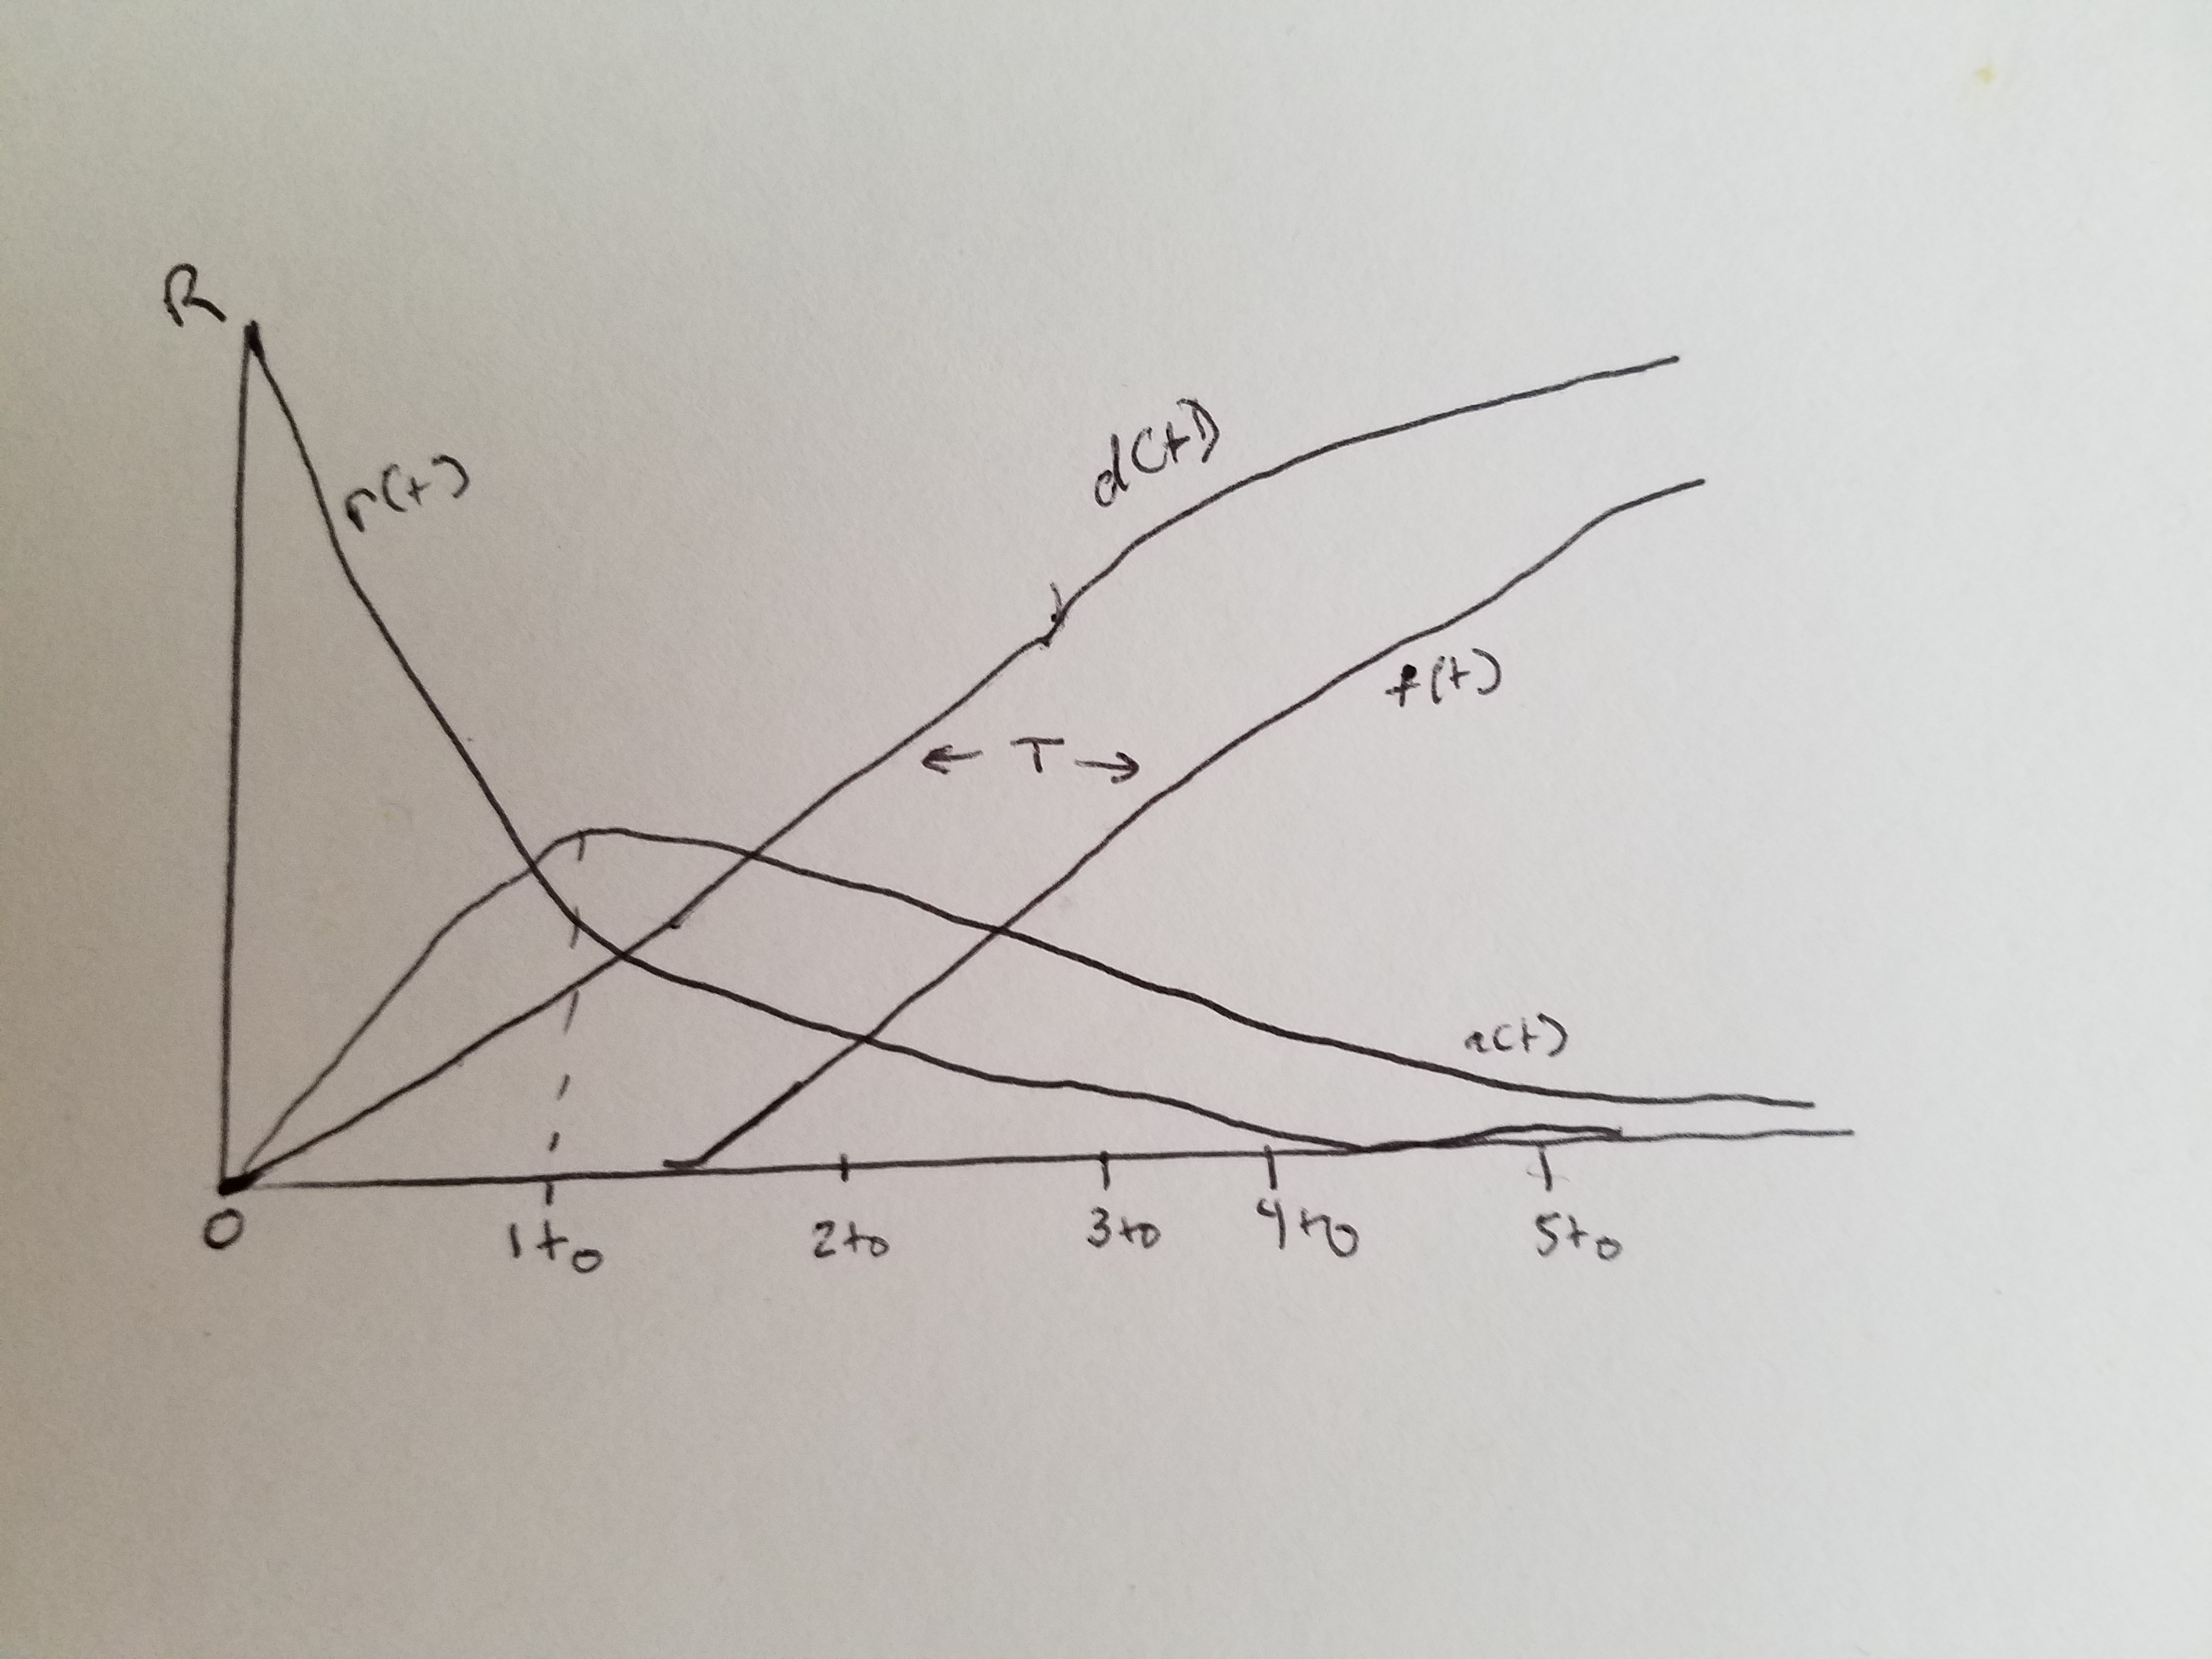
\includegraphics{https://raw.githubusercontent.com/dbouquin/DATA_609_final/master/20170507_152919.jpg}
\newpage

\subsection{Exercise 9.}\label{exercise-9.}

Assuming that increased stay in the digestive system implies improved
digestion determine from Figure 4 which method of food preparation is
more desirable. Why?

\begin{figure}[htbp]
\centering
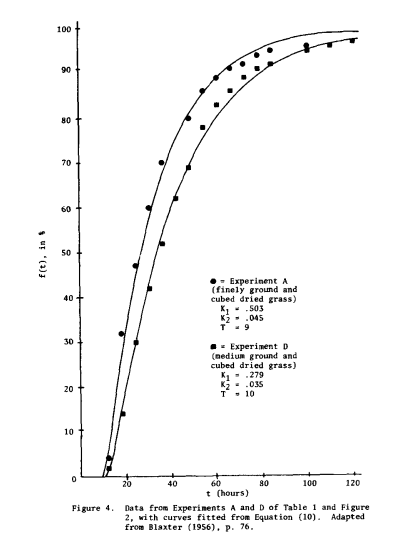
\includegraphics{https://raw.githubusercontent.com/dbouquin/DATA_609_final/master/Figure4.PNG}
\caption{}
\end{figure}

Assuming that we are looking for the feed type that stays in the sheep's
stomach the longest, then we would say that the medium-ground grass
would be the most desirable. We make this assumption as it stands that
the sheep requires less feed for the same results.


\end{document}
